\documentclass[11pt]{article}
\usepackage{../EllioStyle}
\usepackage{fancyvrb}

\title{Homework 2}
\author{Elliott Pryor}
\date{3 Sept 2020}


\begin{document}
\maketitle

\section*{A}

\problem{1}

\begin{figure}[H]
    \centering
    \begin{subfigure}{0.28\textwidth}
		\centering
		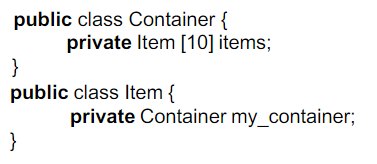
\includegraphics[width=\textwidth]{./pics/prob1_prob.png}
		\caption{Psudocode for problem 1 (QUESTION)}
		\label{fig:prob1_prob}
	\end{subfigure}
	\begin{subfigure}{0.7\textwidth}
		\centering
		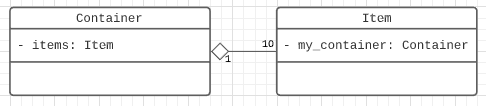
\includegraphics[width=\textwidth]{./pics/prob1_sol.png}
		\caption{UML Diagram for problem 1 (SOLUTION)}
		\label{fig:prob1_sol}
	\end{subfigure}
    \caption{Problem 1 question and solution}
    \label{fig:prob1}
\end{figure}

\problem{2}
\begin{figure}[H]
    \centering
    \begin{subfigure}{0.28\textwidth}
		\centering
		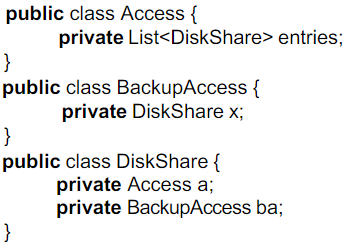
\includegraphics[width=\textwidth]{./pics/prob2_prob.png}
		\caption{Psudocode for problem 2 (QUESTION)}
		\label{fig:prob2_prob}
	\end{subfigure}
	\begin{subfigure}{0.7\textwidth}
		\centering
		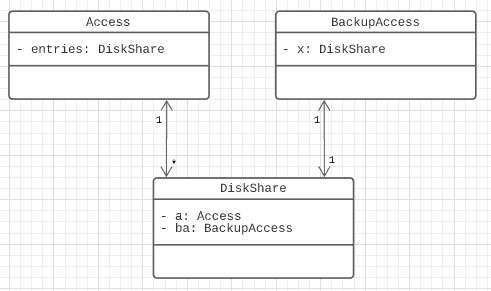
\includegraphics[width=\textwidth]{./pics/prob2_sol.png}
		\caption{UML Diagram for problem 2 (SOLUTION)}
		\label{fig:prob2_sol}
	\end{subfigure}
    \caption{Problem 2 question and solution}
    \label{fig:prob1}
\end{figure}

\problem{3}

\begin{figure}[H]
    \centering
    \begin{subfigure}{0.28\textwidth}
		\centering
		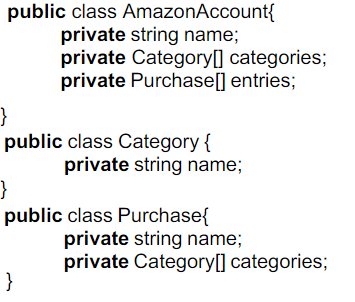
\includegraphics[width=\textwidth]{./pics/prob3_prob.png}
		\caption{Psudocode for problem 3 (QUESTION)}
		\label{fig:prob3_prob}
	\end{subfigure}
	\begin{subfigure}{0.7\textwidth}
		\centering
		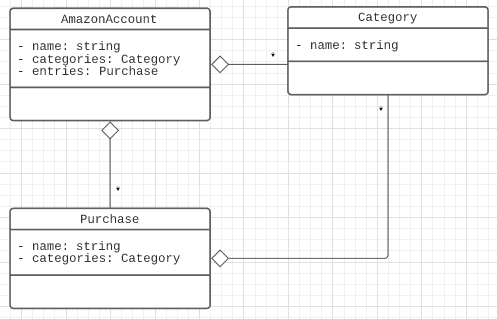
\includegraphics[width=\textwidth]{./pics/prob3_sol.png}
		\caption{UML Diagram for problem 3 (SOLUTION)}
		\label{fig:prob3_sol}
	\end{subfigure}
    \caption{Problem 3 question and solution}
    \label{fig:prob1}
\end{figure}

\problem{4}
\begin{figure}[H]
    \centering
    \begin{subfigure}{0.5\textwidth}
		\centering
		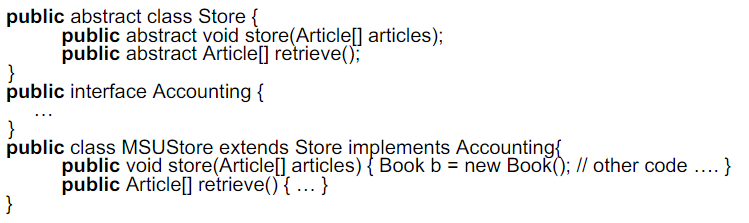
\includegraphics[width=\textwidth]{./pics/prob4_prob.png}
		\caption{Psudocode for problem 4 (QUESTION)}
		\label{fig:prob4_prob}
	\end{subfigure}
	\begin{subfigure}{0.7\textwidth}
		\centering
		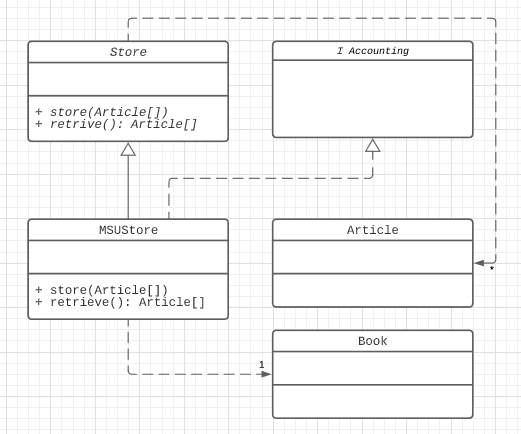
\includegraphics[width=\textwidth]{./pics/prob4_sol.png}
		\caption{UML Diagram for problem 4 (SOLUTION)}
		\label{fig:prob4_sol}
	\end{subfigure}
    \caption{Problem 4 question and solution}
    \label{fig:prob1}
\end{figure}

\newpage
\section*{B}
\begin{Verbatim}
public class Company{
	public string name;
	public Address headquarters;
	public Employee[] employee;
	public Customer[] customer;
	public VehicleRentalService service;
	public Truck[] truck;
	public Car[] car;
	public Motorbike[] motorbike;
}

public abstract class Person{
	public string name;
	public string email;
	public Address address;
}

public class Employee extends Person{
}

public class Customer extends Person{
	public BankAccount bankAccount;
}

public class Subcontractor extends Employee, Person{
}

public class Address{
	public string name;
	public string postalCode;
	public string city;
}

public class BankAccount{
	public int number;
	public string depositor;
	public string bank;
}

public abstract class Service{
	public Customer customer;
}

public class VehicleRentalService extends Service{
	public Vehicle vehicle;
	
	public void offerCar(){}
	public void offerMotorbike(){}
	public void offerTruck(){}
}

public interface Rentable{
	public void rent();
}

public abstract class Vehicle implements Rentable{

	public abstract void rent(); // push implementation to subclasses

}

public class Truck extends Vehicle{
	public int weight;
	public int power;
	public string manufacturer;
	public string regNo;

	public void rent(){}

}

public class Car extends Vehicle{
	public CarKind kind;
	public int noSeats;
	public int power;
	public string manufacturer;
	public string regNo;

	public void rent(){}
}

public class Motorbike extends Vehicle{
	public MbKind kind;
	public int cylinderCap;
	public int power;
	public string manufacturer;
	public string regNo;

	public void rent(){}
}




\end{Verbatim}

\end{document}